% Asset ID: A21ParametricEquationsTikZ-005
% Source: Transcript points of intersection section; CCEA A21-CG-LO001.
% Related lesson section: Worked Example 6; Exam Technique Notes.
% Purpose: Show substitution into a line, solve for t, then find coordinates.

\documentclass[tikz,border=8pt]{standalone}
\usepackage{amsmath}
\usepackage{pgfplots}
\pgfplotsset{compat=1.18}
\begin{document}
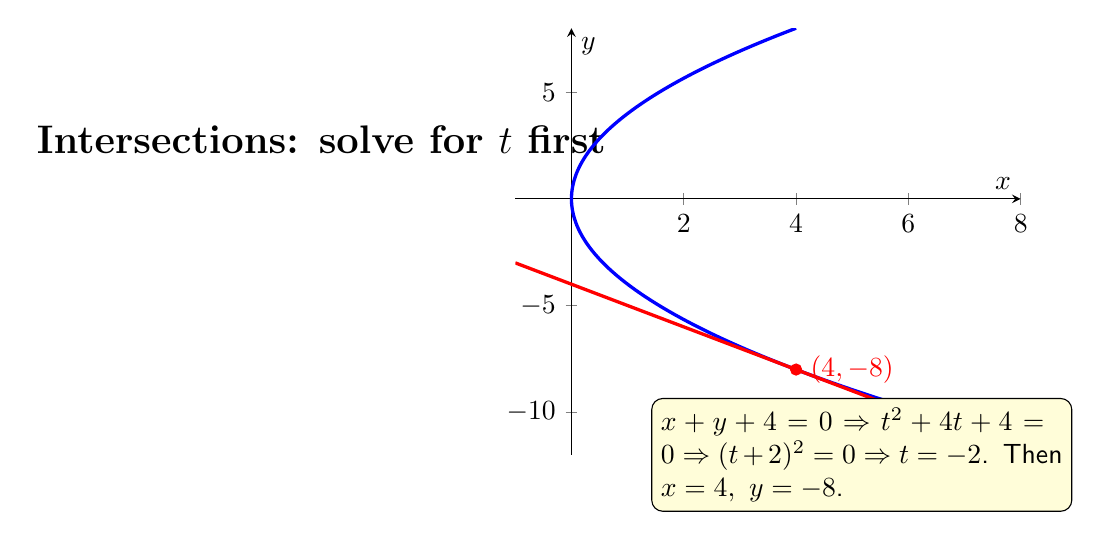
\begin{tikzpicture}[font=\sffamily]

\node[anchor=west, font=\bfseries\Large] at (-6.2,4.0) {Intersections: solve for \(t\) first};
\begin{axis}[width=8cm,height=7cm,axis lines=middle,xmin=-1,xmax=8,ymin=-12,ymax=8,xlabel={$x$},ylabel={$y$}]
\addplot[domain=-3:2,samples=120,blue,very thick] ({x^2},{4*x});
\addplot[domain=-1:8,samples=2,red,very thick] {-x-4};
\addplot[only marks,red] coordinates {(4,-8)};
\node[red] at (axis cs:5,-8) {\((4,-8)\)};
\end{axis}
\node[draw, rounded corners, fill=yellow!15, text width=5.1cm] at (4.4,0) {\(x+y+4=0\Rightarrow t^2+4t+4=0\Rightarrow(t+2)^2=0\Rightarrow t=-2\). Then \(x=4,\ y=-8\).};

\end{tikzpicture}
\end{document}
